\documentclass[final]{beamer}
\mode<presentation>

\usetheme{I6dv}

\usepackage{amsmath,amsthm, amssymb}
%\usepackage{algorithmic}
\usepackage{algorithm}
\usepackage{algpseudocode}

\usepackage{exscale}

%\usepackage[caption=false]{subfig}
\usepackage[compatibility=false]{caption}
\usepackage{subcaption}


\usepackage[orientation=landscape,size=a0,scale=1.4]{beamerposter}

\setbeamertemplate{caption}[numbered]

\title{\Huge An Introduction to Elliptic Curve Cryptography}
\author{Tanner Prynn}
\institute{The University of Arizona}
\date{Aug. 31 , 2007}

\begin{document}
\begin{frame}{} 
	\vskip-1ex
	\begin{columns}[t]

	\begin{column}{.3\linewidth}

	\begin{block}{Elliptic Curves}
		An \textbf{elliptic curve} is a set of points satisfying an equation of the form
		$$y^2 = x^3 + ax + b$$
		for coefficients $a,b$ and variables $x,y$ in some field $F$ (of characteristic not 2 or 3). 
		This type of equation is a Weierstrass equation, which is a condensed form of a general cubic equation.
		One additional restriction is placed on an elliptic curve, which is that
		$4a^3 + 27b^2 \neq 0$.
		This condition ensures that the curve is \textit{non-singular}, which allows us to find a tangent line to any point on the curve.

		Figure \ref{fig:ec-plot} shows a simple elliptic curve.

		\begin{figure}[h]
		\centering
		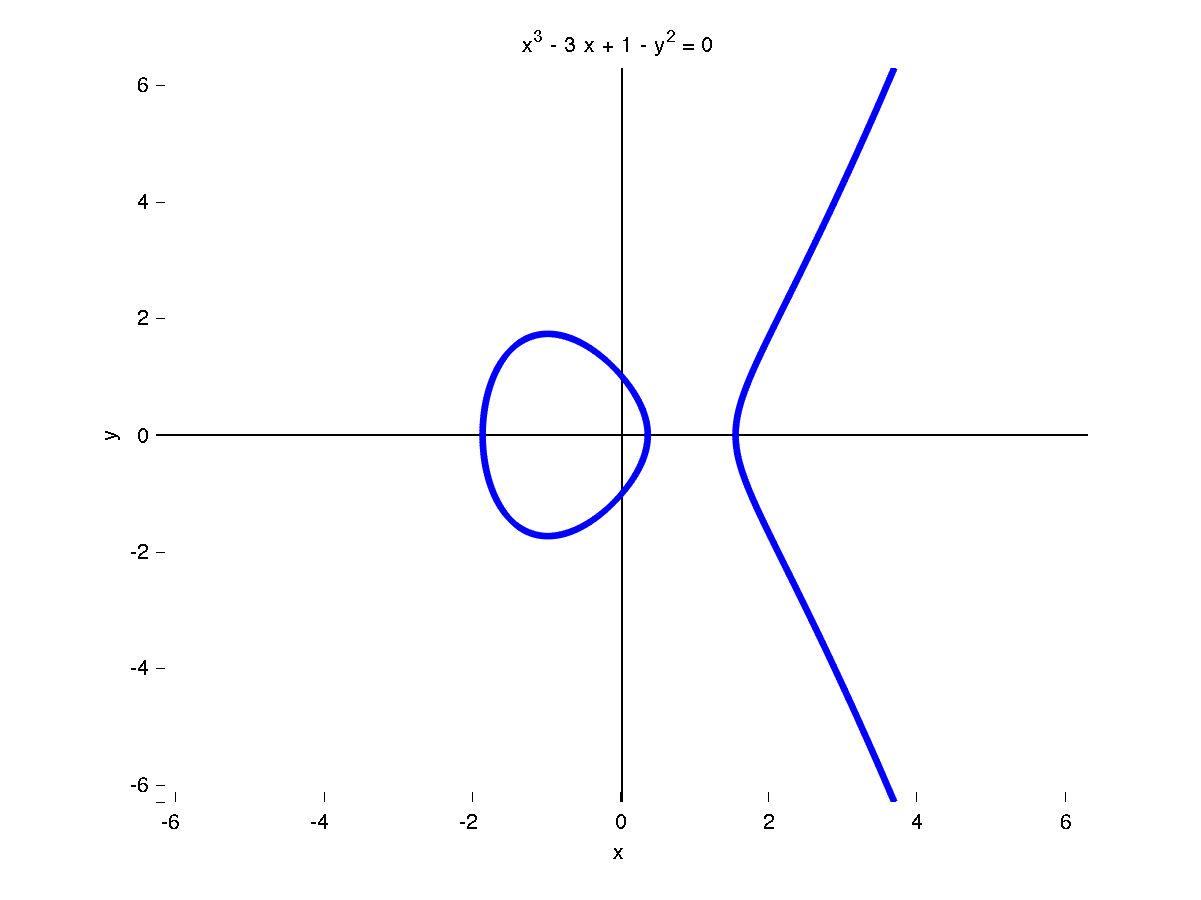
\includegraphics[width=0.7\linewidth]{../images/ec1.png}
		\caption{The elliptic curve $y^2 = x^3 - 3x + 1$}
		\label{fig:ec-plot}
		\end{figure}

	\end{block}

	\vskip1ex

	\begin{block}{The Group Law}
		Define the set of points on the curve as
		$$C = \{(x,y) \mid x,y \in F \text{ and } y^2 = x^3 + ax + b\} \cup \infty$$%
		where $\infty$ is the point at infinity in the projective plane.

		There is an operation $+$ which allows the composition of any two points on the curve.
		Figure \ref{fig:ec-plus} shows the geometric application of this operation.

		\begin{figure}[h]
		\centering

		\begin{subfigure}{.5\linewidth}
			\centering
			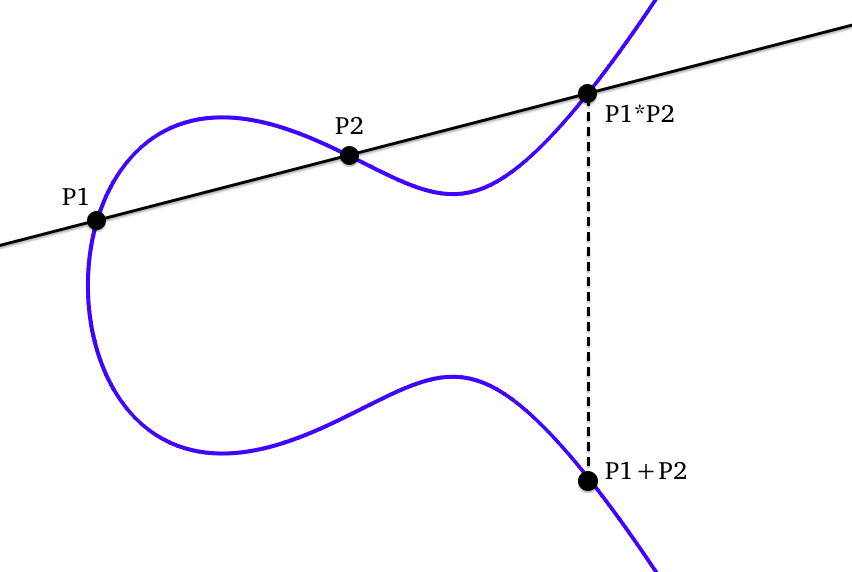
\includegraphics[width=1\linewidth]{../images/ec4-plus.png}
			\label{fig:ec-plus-1}
		\end{subfigure}%
		~%
		\begin{subfigure}{.5\linewidth}
			\centering
			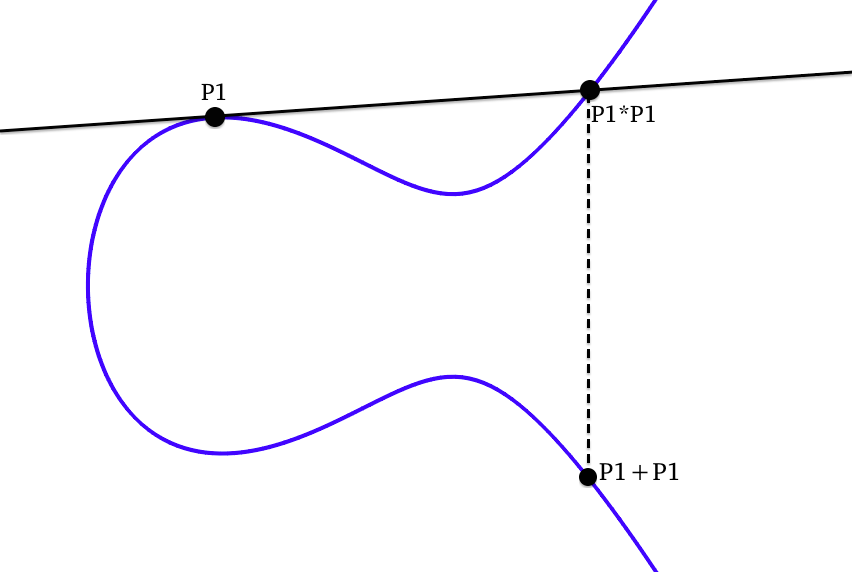
\includegraphics[width=1\linewidth]{../images/ec4-plus-tangent.png}
			\label{fig:ec-plus-2}
		\end{subfigure}

		\caption{The $+$ operation for two points on an elliptic curve}

		\label{fig:ec-plus}
		\end{figure}

		To add two points together, take the line between them and find its third point of intersection with the curve, then reflect across the $x$-axis.
		To add a point to itself, use the tangent line.
		The identity of $+$ is $\infty$. The inverse of a point is its reflection across the $x$-axis.

	\end{block}

	\end{column}

	\begin{column}{.3\linewidth}

	\begin{block}{The Discrete Logarithm Problem}
		Given a group $G$ with operation $*$ we can define a map $\cdot: \mathbb{Z} \times G \to G$ by
		$$n\cdot g \mapsto \underbrace{g * g * \cdots * g}_{n\text{ times}}$$
		On an elliptic curve, the map $\cdot$ is equal to the repeated addition of a point to itself. 
		We call this map \textit{point multiplication}.
		For a point $P$ on $C$, $nP = P + P + \cdots + P$.
		If we have two points $P,Q$ on $C$ where $nP = Q$, then $n$ is the \textit{elliptic-curve discrete logarithm} (ECDL) of $Q$ with respect to $P$.

		Point multiplication is an example of a \textit{trap-door function}: a function which is simple to compute in one direction but difficult to compute in the other direction.
		This is the exact operation we will use to construct a cryptosystem.

		\vskip1ex
        \noindent{\textbf{Naive Multiplication}} \\
		If an attacker knows $P$ and $nP$, where $N$ is the order of $C$, then they can solve the discrete logarithm problem by testing if $mP = nP$ for each $m$, $1 \leq m < N$.
		This is the simplest attack on the ECDLP, and will complete in $O(NM)$ time, where $M$ is the cost of an elliptic curve multiplication.

		For small curves, a computer performing naive multiplication will quickly solve the ECDLP. 
		Generic attacks against the ECDLP all have complexity which is a function of the order of the curve, so cryptographic curves are picked such that their order is very large: more than $2^{200}$.

		\vskip1ex
		\noindent{\textbf{Baby-Step Giant-Step}} \\
		The Baby-Step Giant-Step algorithm rewrites the point $Q = nP$ as $(im + j)P$, with $m = \lceil \sqrt{N} \rceil$.
		Then $jP$ is computed for $0 \leq j < m$ and stored.
		Finally, naive multiplication is used to find $imP$ for $0 \leq i < m$, and subtracted from $nP$ to solve for $jP$.

		\vskip1ex
		\centerline{
		\begin{minipage}{0.8\linewidth}
		\centering
		\begin{algorithm}[H]
		\caption*{Baby-Step Giant-Step for ECDLP}
		\begin{algorithmic}
		\State $m \gets \sqrt{N}$
		\For{$0 \leq j < m$}
			\State Compute and store $(j, jP)$
		\EndFor
		\For{$0 \leq i < m$}
			\State Compute $Q - imP$
			\If{$Q-imP = jP$ for some $j$}
				\State \Return $n \equiv j + im$
			\EndIf
		\EndFor
		\end{algorithmic}
		\end{algorithm}
		\end{minipage}
		}
		\vskip0.5ex

		Baby-Step Giant-Step completes in $O(\sqrt{N} M)$ time and $O(\sqrt{N})$ space complexity.
		This is a large improvement over naive multiplication, but still very slow on cryptographic curves. 
		There is no known algorithm which feasibly solves the ECDLP on a generic cryptographic curve, and this problem is what elliptic curve cryptography is based on.
	\end{block}

	\end{column}

	\begin{column}{.3\linewidth}

	\begin{block}{Elliptic Curve Diffie-Hellman Exchange}
	\end{block}

	\vskip1ex

	\begin{block}{Curve25519}
	\end{block}

	\end{column}

	\end{columns}
\end{frame}{}
\end{document}